\documentclass[10pt]{article}
\usepackage[margin=0.7in]{geometry}
\usepackage[T1]{fontenc}
\usepackage{lmodern,graphicx,booktabs,array,hyperref,fancyhdr}
\hypersetup{colorlinks=true,urlcolor=blue}
\pagestyle{fancy}\fancyhf{}\lhead{Classical prime-field ECDLP}\rhead{23 November 2026}
\cfoot{Producer records: PCC unverified --- \thepage}
\setlength{\headheight}{14pt}\setlength{\parindent}{0pt}\setlength{\parskip}{5pt}
\setlength{\emergencystretch}{3em}
\begin{document}
{\Large\bfseries Complete CPU public-target validation through 40-bit fields}

The existing native CPU pipeline completed \textbf{24 of 24 calls on 12 distinct
public targets}, with every original external certificate replay passing.
All 12 identical-arm certificate pairs are byte-identical. The two seeds are
different targets on each curve. Unsigned observations are registered as
\texttt{PCC-20261123-e8d860}; this report does not supply a signed execution verdict.

\begin{center}
\begin{tabular}{@{}rrrrrr@{}}\toprule
Field bits & Order bits & Targets & Calls & Relations & Attempts\\\midrule
20&20&2&4/4&49--57&57--60\\
24&25&2&4/4&71--79&80--86\\
28&28&2&4/4&105--109&106--111\\
32&32&2&4/4&128--136&185--215\\
36&36&2&4/4&178--183&300--380\\
40&41&2&4/4&267--280&332--380\\\bottomrule
\end{tabular}
\end{center}
Counts and per-target ranges come from the original rows. Both A/A arms are
retained; they do not double the number of distinct targets. Field size and
prime subgroup-order size are stated separately.

\textbf{Prospective protocol.} Protocol version2 was committed at
\texttt{c691d21db7a03726e06c6ae1c0b542cdc0ce38c3} before affected data.
Its canonical SHA256 is\par
{\footnotesize\texttt{f4154a35224588ece8fd2b6a6c6d089a95907c9f1c5e468322c2098e88350bad}.}
The inherited six curves, seeds 101/202, eight slots, batch size 64, 20M rows,
max\_trials 16 and max\_columns 16384 remain. Targets are the first decodable
even-y point starting at \texttt{x=seed*1009 mod p}; no scalar is constructed
or supplied. The implementation is the existing generic-decomposition
\texttt{CachedMitm} CPU pipeline.

\textbf{Flow and limits.} Original limits are 120s per call, 60s per external
replay, 1500s total, one attempt, stopping before the next level after any cell
failure. All 24 were attempted and verified; failed 0, unattempted 0. The original
primary analyzer and raw session remain unchanged.

\textbf{Local conditions.} Workload interval 11:55:37--11:56:53 UTC; one worker
under the shared lock; no concurrent builds/tests. A 4GiB virtual-address limit
is distinct from RSS. Sampled whole-cgroup peak 13,337,882,624 bytes includes
unrelated retained research; guard 15,032,385,536 bytes; no physical stop.
Clocks are L0 diagnostics. No capacity purchase, external spend or S3 upload.

\textbf{Qualification.} Original Rust 1.99.1 build and 47 native checks pass,
zero failed/ignored; one empty harness. All 108 source/input digests and seven
frozen executable identities match after the cohort. Build source is
\texttt{cc893a73}; run checkout is \texttt{c691d21d}; crypto source is identical.
The compiler checkout had an unrelated journal edit: export source cleanliness
refers to the pinned program/input set, not that journal.

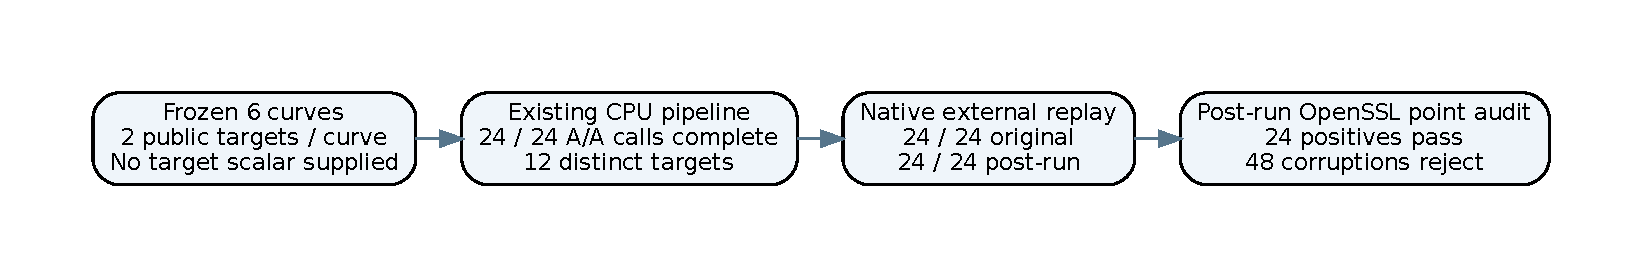
\includegraphics[width=\linewidth,height=1.5in,keepaspectratio]{validation-flow.pdf}

\newpage
{\Large\bfseries Frozen primary plot and measurement boundary}

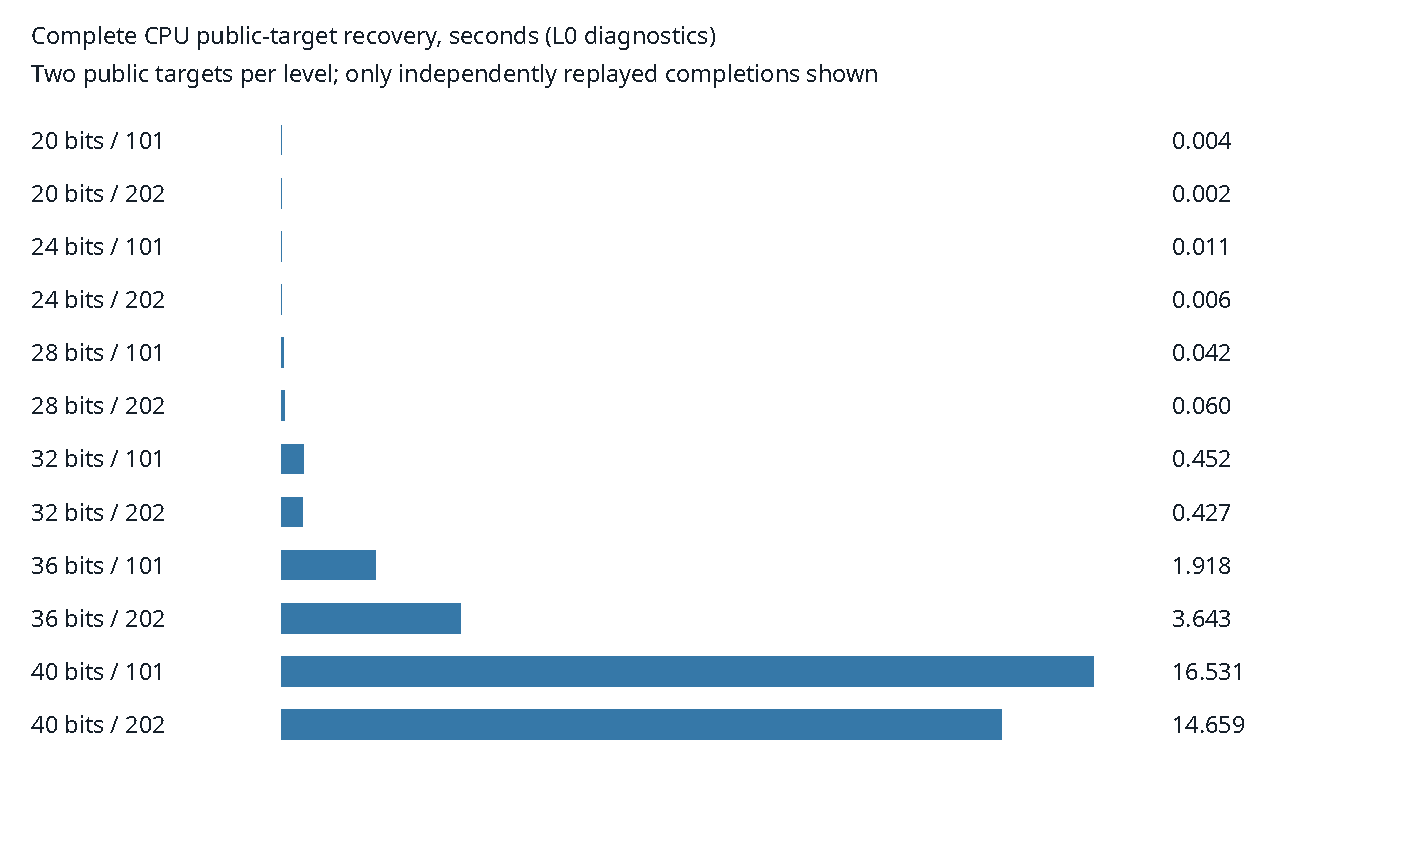
\includegraphics[width=\linewidth]{scale.pdf}

\textbf{Figure.} Unchanged SVG from the frozen native analyzer for
\texttt{HASHED-ECDL-CPU-SCALE-LOCAL-20261123}. Twelve u-arm observations,
two distinct public targets per field size; all 24 u/x rows remain published.
Units are seconds. No uncertainty interval was recorded. Separate-process
Native replay is what the inherited label ``independently replayed'' describes;
it is not a claim of independent actor or signed provenance.

\textbf{Clock boundary.} Complete internal clock includes curve/public-target
construction, trial/base/table preparation, all relation attempts, elimination,
internal replay, Archive verification and serialization. It excludes file I/O,
process launch and the external replay process. OpenSSL audits run afterwards.
The exported table capacity is retained prefix/suffix capacity, not process RSS.
CPU time and per-call peak RSS are missing, not zero.

\textbf{Interpretation.} This is a complete-recovery feasibility cohort of an
existing solver. It supplies no matched candidate/reference, calibrated common
operation price, inferential speed comparison, exponent fit or extrapolation.
The two A/A executions do not provide independent target samples. The separate
84-case tensor panel and its original deadline remain unchanged.

\textbf{Reproduction inputs.} The study's protocol, original Rust analyzer,
unchanged parent runner, thin local launcher, build/pre-call/post-call manifests
and qualified binary hashes bind the run. Compact rows, status, native replay
outputs and post-run controls accompany this report. Full JSON certificates,
exports and qualified binaries are retained locally with SHA256 receipts.

\newpage
{\Large\bfseries Post-run validation, corrections and next comparison}

\begin{tabular}{@{}p{0.29\linewidth}p{0.65\linewidth}@{}}\toprule
Check & Recorded observation and boundary\\\midrule
Original Native replay &24/24 certificates pass in external processes.\\
Post-run Native replay &24/24 additional Archive replays pass.\\
OpenSSL positives &24/24 public-target bindings, nonidentity, \texttt{rP=O}, \texttt{kP=Q} pass.\\
Wrong scalar &24/24 reject specifically at \texttt{SCALAR kP=Q}.\\
Consistent substitution &24/24 pairs \texttt{(r-k,-Q)} reject specifically at \texttt{BINDING public target}.\\
Lossless metadata &Seven regression/whitelist checks and strict all-target Clippy pass; final canonical check has zero findings.\\\bottomrule
\end{tabular}

These audits were added after data and do not replace the frozen primary
analysis. OpenSSL 3.5.7 uses separate point arithmetic, explicit bitwise
double/add and no installed group-order metadata. It reconstructs the fixed
public target before checking the scalar. Its 256-position target-search bound
admits all recorded fixtures. It does not independently prove primality,
Hasse cardinality, full relation certificates, work counters or execution history.
Full Native replay shares solver arithmetic. Read-only artifact review is
distinct from an independently signed execution or validator attestation.

\textbf{Preserved failures.} Original export uses replicate 0 for both seeds:
12 duplicate canonical keys. Preserved v2 repairs keys but rounds five timing
values; review 06 rejects exact preservation despite schema acceptance. The
separate arbitrary-precision adapter preserves all numeric lexemes and checks
the complete recursive delta. Initial test 08 failed because its synthetic
fixture omitted existing header fields; corrected 08b passes 7/7. All failures
and both original exports remain. V3's manually supplied future creation header
was preserved; final v3b uses actual current UTC, differing only in that header.

Final v3b is 123,081 bytes, SHA256\par
{\footnotesize\texttt{07a7f73eeecf1ed24cfb203233982135235e90b82822bc896ccefdabe1e5d208}.}
Review finds 39 allowed original-to-final metadata changes, zero measurement,
artifact, outcome, seed or protocol drift. Slots 0/1 identify the distinct declared
targets. Earlier reviews and all 340 input-manifest entries remain immutable.

\textbf{Publication boundary.} User excludes S3. Oversized data stays local;
\texttt{DATA-RECEIPT.json} pins complete exports/certificates. The remote PR alone
does not include the full replay payload. A verified local handoff capsule is
recorded separately after the result snapshot. Signed PCC execution standing
and full-root/MSRV gates are not established here.

\textbf{Next discriminating experiment.} Reconcile an actually distinct,
reachable CPU candidate and its current comparator before freezing matched
cold-recovery and common-cost controls. Report component or whole-pipeline
improvements at the measured scope. Preserve the separate tensor source/history
and total-cost proof obligations and original 84-case acceptance.

\textbf{Sources.} Existing CPU solver/certificate/scale and shared reduction
sources; inherited CPU scale runner/analyzer; round 24/25 proposals; captured
canonical protocol/schema; OpenSSL 3.5 EC\_POINT documentation. KB tools were
unavailable (wrapper 127); live sibling text reads failed UTF8 decoding.
No novelty clearance follows. Canonical leaderboard/ranking graphs remain
unchanged because no comparative gate-qualified entry is supplied.

\small Source-linked outcome: \path{research/hashed_ecdl_cpu_scale_20261123/OUTCOME.md}.\par
\url{https://github.com/isogeny-labs/crypto/pull/4996}
\end{document}
